\documentclass[12pt]{article}
\usepackage[utf8]{inputenc}
\usepackage[T1]{fontenc}
\usepackage{geometry}
\geometry{margin=1in}
\usepackage{hyperref}
\usepackage{tikz}
\usepackage{pgfplots}
\usepackage{algorithm}
\usepackage{algpseudocode}
\usepackage{amsmath}
\usepackage{amssymb}
\usepackage{graphicx}
\usepackage{listings}
\usepackage{xcolor}
\usepackage{float}
\usepackage{tabularx}
\usetikzlibrary{shapes,arrows,positioning,calc,backgrounds,fit}
\pgfplotsset{compat=1.18}
\title{Sistema Distribuido P2P con Topología Hipercubo}
\author{Abel Ponce González C411\\Richard Alejandro Matos Arderí C411}
\date{\today}

\begin{document}

\maketitle

\begin{abstract}
Este documento presenta la especificación arquitectónica de un sistema distribuido peer-to-peer descentralizado basado en topología hipercubo. Se detalla la arquitectura del sistema, la organización y roles de sus componentes, los procesos y patrones de diseño implementados, los mecanismos de comunicación y coordinación, el sistema de nombrado y localización de recursos, las estrategias de consistencia y replicación, los mecanismos de tolerancia a fallos y los aspectos de seguridad del diseño.
\end{abstract}

\tableofcontents

\newpage

\section{Introducción}

\subsection{Descripción del sistema}
El sistema propuesto es una plataforma distribuida peer-to-peer para almacenamiento y consulta de información de forma descentralizada. Utiliza una topología de red overlay tipo hipercubo que estructura la organización lógica de los nodos, proporcionando rutas eficientes de comunicación, redundancia y tolerancia a fallos.

\subsection{Objetivos del diseño}
\begin{itemize}
  \item Eliminar puntos únicos de fallo mediante una arquitectura completamente descentralizada
  \item Garantizar alta disponibilidad de datos mediante replicación estratégica
  \item Proporcionar mecanismos eficientes de localización de recursos sin índices centralizados
  \item Implementar tolerancia a fallos con recuperación automática
  \item Asegurar comunicaciones mediante protocolos de seguridad robustos
\end{itemize}

\section{Arquitectura del Sistema}

\subsection{Estilo arquitectónico}

\subsubsection{Clasificación según estilos arquitectónicos}

El sistema sigue un \textbf{estilo arquitectónico peer-to-peer estructurado} que se caracteriza por una organización simétrica de componentes con capacidades equivalentes. Los componentes principales son nodos peer que exponen interfaces bien definidas para operaciones de almacenamiento, consulta y routing. Cada componente encapsula datos y ofrece métodos sin revelar su implementación interna, siguiendo el estilo basado en objetos. Esta encapsulación permite que los componentes sean reemplazables mientras mantengan la interfaz estándar del sistema.

La comunicación entre componentes se realiza mediante conectores que incluyen sockets TCP/UDP para comunicación punto a punto confiable, mecanismos de mensajería asíncrona para coordinación entre nodos, y streaming de datos para transferencias grandes. La configuración del sistema está determinada por una topología overlay hipercubo que define las conexiones lógicas entre nodos, creando una red estructurada con un índice distribuido basado en direcciones binarias.

\subsection{Modelo arquitectónico: P2P estructurado descentralizado}

\subsubsection{Características del sistema P2P}

El sistema implementa una arquitectura peer-to-peer \textbf{estructurada} pura sin componentes centralizados. La característica fundamental es la simetría de roles: cada nodo peer actúa simultáneamente como cliente y servidor (patrón servant). Esto significa que un mismo nodo puede iniciar consultas hacia otros peers (actuando como cliente) y al mismo tiempo atender solicitudes de otros nodos (actuando como servidor). No existe distinción funcional entre los nodos; todos tienen capacidades equivalentes para almacenar fragmentos de datos y réplicas, procesar consultas tanto propias como de otros nodos, reenviar peticiones según algoritmos de routing, participar en protocolos de replicación y consistencia, y mantener conexiones activas con sus vecinos lógicos en la topología.

El sistema utiliza un índice distribuido semánticamente libre donde cada dato se asocia con una clave única derivada de las direcciones binarias en el hipercubo. El sistema emplea direccionamiento directo basado en la estructura del hipercubo, donde cada nodo es responsable de mantener pares (clave, valor) que corresponden a su región del espacio de direcciones. Esto crea un índice distribuido sin necesidad de un servidor central de índices, aprovechando las propiedades geométricas del hipercubo para routing eficiente.

\begin{figure}[H]
\centering
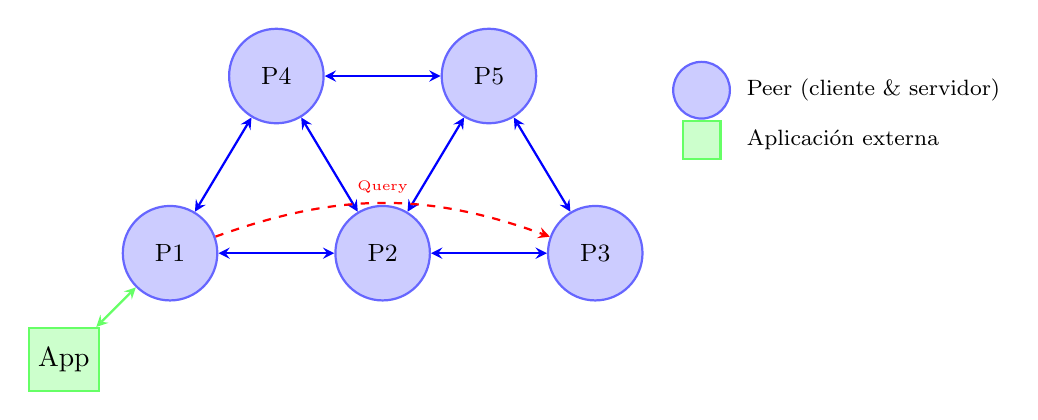
\begin{tikzpicture}[scale=0.9]
  % Definir estilos
  \tikzstyle{peer}=[circle, draw=blue!60, fill=blue!20, thick, minimum size=1.2cm, font=\small]
  \tikzstyle{extclient}=[rectangle, draw=green!60, fill=green!20, thick, minimum size=0.8cm]
  \tikzstyle{conn}=[<->, thick, >=stealth]
  \tikzstyle{query}=[->, thick, >=stealth, red, dashed]
  
  % Nodos peer (todos son clientes Y servidores)
  \node[peer] (p1) at (0,0) {P1};
  \node[peer] (p2) at (3,0) {P2};
  \node[peer] (p3) at (6,0) {P3};
  \node[peer] (p4) at (1.5,2.5) {P4};
  \node[peer] (p5) at (4.5,2.5) {P5};
  
  % Cliente externo (aplicación sin capacidad de servidor)
  \node[extclient] (c1) at (-1.5,-1.5) {App};
  
  % Conexiones P2P (cada peer puede ser cliente del otro)
  \draw[conn, blue] (p1) -- (p2);
  \draw[conn, blue] (p2) -- (p3);
  \draw[conn, blue] (p1) -- (p4);
  \draw[conn, blue] (p2) -- (p4);
  \draw[conn, blue] (p2) -- (p5);
  \draw[conn, blue] (p3) -- (p5);
  \draw[conn, blue] (p4) -- (p5);
  
  % Ejemplo: P1 inicia consulta hacia P3 (P1 actúa como cliente)
  \draw[query] (p1) to[bend left=20] node[above, font=\tiny] {Query} (p3);
  
  % Cliente externo se conecta a cualquier peer
  \draw[conn, green!60] (c1) -- (p1);
  
  % Leyenda
  \node[peer, scale=0.6] at (7.5,2.3) {};
  \node[right, font=\footnotesize] at (8,2.3) {Peer (cliente \& servidor)};
  \node[extclient, scale=0.6] at (7.5,1.6) {};
  \node[right, font=\footnotesize] at (8,1.6) {Aplicación externa};
\end{tikzpicture}
\caption{Arquitectura P2P: cada peer actúa como cliente y servidor. P1 puede consultar a P3 (cliente) mientras atiende peticiones de otros (servidor)}
\label{fig:p2p-arch}
\end{figure}

\subsection{Distribución del sistema}

\subsubsection{Distribución horizontal}
El sistema emplea \textbf{distribución horizontal} (horizontal distribution), donde los nodos peer están físicamente distribuidos en múltiples máquinas pero mantienen capacidades equivalentes. Cada nodo opera sobre su propio subconjunto del conjunto completo de datos, sin que exista una jerarquía vertical de capas entre los peers. Todos los nodos ejecutan el mismo software y pueden asumir cualquier rol necesario, lo que garantiza simetría funcional en el sistema. Esta distribución horizontal contrasta con la distribución vertical (donde diferentes capas de aplicación residen en diferentes máquinas), enfatizando la naturaleza descentralizada de la arquitectura P2P.

\subsection{Topología de red overlay: Hipercubo estructurado}

\subsubsection{Definición de la topología}
La red lógica (overlay) se estructura como un hipercubo de dimensión $d$. En esta topología, cada nodo posee una dirección binaria única de $d$ bits que determina su posición en el espacio lógico. Los vecinos lógicos de un nodo son aquellos cuya dirección difiere en exactamente un bit, lo que significa que cada nodo mantiene $d$ conexiones directas. El número máximo de nodos que puede soportar el sistema es $N = 2^d$, y la distancia máxima entre cualquier par de nodos (diámetro de la red) es también $d$.

Esta estructura presenta propiedades clave que la hacen ideal para sistemas distribuidos. La \textbf{conectividad} múltiple garantiza redundancia, ya que existen varias rutas alternativas entre cualquier par de nodos. La \textbf{escalabilidad} se manifiesta en el crecimiento logarímico del diámetro respecto al número de nodos, lo que mantiene las latencias manejables incluso con miles de nodos. La \textbf{simetría} asegura que todos los nodos tienen el mismo grado de conectividad, evitando cuellos de botella. Finalmente, la \textbf{tolerancia a fallos} se logra porque la red permanece conectada incluso ante fallos de nodos individuales, gracias a las rutas alternativas disponibles.

\subsubsection{Ejemplo: Hipercubo de dimensión 3}
Un hipercubo de dimensión 3 (\(d=3\)) tiene \(2^3 = 8\) nodos, cada uno con una dirección binaria de 3 bits (000, 001, 010, ..., 111). Cada nodo tiene exactamente 3 vecinos (uno por cada bit que puede cambiar).

\begin{figure}[H]
\centering
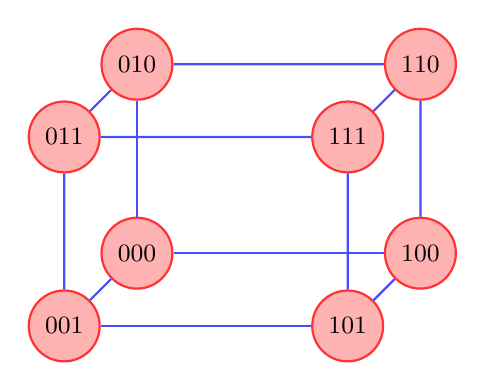
\begin{tikzpicture}[scale=1.2]
  \tikzstyle{node}=[circle, draw=red!80, fill=red!30, thick, minimum size=0.9cm, font=\small]
  \tikzstyle{edge}=[-, thick, blue!70]
  
  % Vértices del cubo (hipercubo 3D)
  \node[node] (n000) at (0,0,0) {000};
  \node[node] (n001) at (0,0,2) {001};
  \node[node] (n010) at (0,2,0) {010};
  \node[node] (n011) at (0,2,2) {011};
  \node[node] (n100) at (3,0,0) {100};
  \node[node] (n101) at (3,0,2) {101};
  \node[node] (n110) at (3,2,0) {110};
  \node[node] (n111) at (3,2,2) {111};
  
  % Aristas del cubo
  \draw[edge] (n000) -- (n001);
  \draw[edge] (n000) -- (n010);
  \draw[edge] (n000) -- (n100);
  \draw[edge] (n001) -- (n011);
  \draw[edge] (n001) -- (n101);
  \draw[edge] (n010) -- (n011);
  \draw[edge] (n010) -- (n110);
  \draw[edge] (n011) -- (n111);
  \draw[edge] (n100) -- (n101);
  \draw[edge] (n100) -- (n110);
  \draw[edge] (n101) -- (n111);
  \draw[edge] (n110) -- (n111);
\end{tikzpicture}
\caption{Hipercubo de dimensión 3: cada nodo tiene 3 vecinos (difieren en 1 bit)}
\label{fig:hypercube3d}
\end{figure}

\subsubsection{Propiedades matemáticas del hipercubo}
Para un hipercubo de dimensión \(d\):
\begin{itemize}
  \item \textbf{Número de nodos}: \(N = 2^d\)
  \item \textbf{Grado de cada nodo}: \(d\) (cada nodo tiene \(d\) vecinos)
  \item \textbf{Diámetro de la red}: \(d\) (máximo número de saltos entre dos nodos cualesquiera)
  \item \textbf{Número total de aristas}: \(\frac{N \cdot d}{2} = d \cdot 2^{d-1}\)
  \item \textbf{Conectividad}: \(d\) (número de caminos disjuntos entre nodos)
\end{itemize}

\textbf{Ejemplo de routing}: Para enviar un mensaje del nodo 000 al nodo 111:
\begin{enumerate}
  \item Comparar direcciones bit a bit: 000 vs 111 $\rightarrow$ difieren en 3 bits
  \item Ruta posible: 000 $\rightarrow$ 100 $\rightarrow$ 110 $\rightarrow$ 111 (3 saltos)
  \item Existen múltiples rutas alternativas de longitud 3
\end{enumerate}

\section{Roles y organización funcional}

En el sistema P2P propuesto, el concepto de "rol" es fluido debido a la naturaleza simétrica de la arquitectura. El componente fundamental es el \textbf{nodo peer}, que simultáneamente actúa como cliente y servidor. Cuando un peer necesita localizar un dato que no posee localmente, asume el rol de \textbf{cliente} iniciando consultas hacia otros peers. Al mismo tiempo, ese mismo peer puede estar atendiendo solicitudes de otros nodos, actuando como \textbf{servidor}. Esta dualidad cliente-servidor es la esencia del modelo peer-to-peer y permite que el sistema funcione sin depender de servidores dedicados.

Cuando un peer almacena datos, responde peticiones y participa en el routing de mensajes, está ejerciendo su rol de servidor. Cuando ese mismo peer busca información, solicita datos a otros nodos o envía consultas a través de la red, está ejerciendo su rol de cliente. Es importante destacar que estas funciones no son excluyentes sino concurrentes: un peer puede estar procesando múltiples peticiones entrantes (servidor) mientras simultáneamente envía sus propias consultas a otros nodos (cliente).

Adicionalmente, el sistema  posee un \textbf{balanceo de carga} que esta lógica no constituye un servidor central sino un algoritmo que cada peer utiliza para tomar decisiones sobre cómo distribuir sus peticiones entre vecinos, considerando factores como carga actual, latencia y disponibilidad. Esto lo asume un pequeño conjunto de peers tomando responsabilidades adicionales de coordinación de manera redundante, sin romper la descentralización del sistema.

\subsection{Diagrama de roles e interacciones}

\begin{figure}[H]
\centering
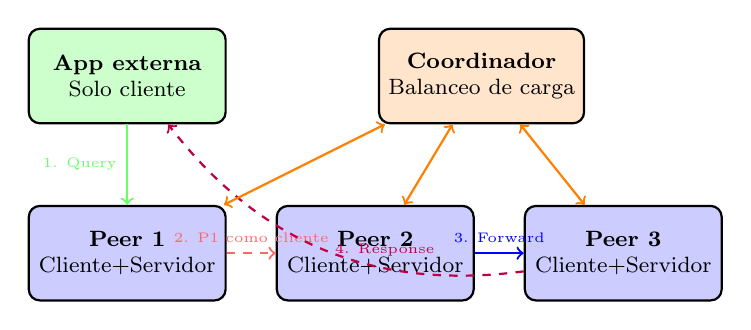
\begin{tikzpicture}[scale=0.9]
  \tikzstyle{role}=[rectangle, draw, thick, minimum width=2.5cm, minimum height=1.2cm, rounded corners, font=\footnotesize, align=center]
  \tikzstyle{peer}=[role, fill=blue!20]
  \tikzstyle{app}=[role, fill=green!20]
  \tikzstyle{coord}=[role, fill=orange!20]
  
  \node[app] (c) at (0,4) {\textbf{App externa}\\Solo cliente};
  \node[coord] (coord) at (5,4) {\textbf{Coordinador}\\Balanceo de carga};
  \node[peer] (p1) at (0,1.5) {\textbf{Peer 1}\\Cliente+Servidor};
  \node[peer] (p2) at (3.5,1.5) {\textbf{Peer 2}\\Cliente+Servidor};
  \node[peer] (p3) at (7,1.5) {\textbf{Peer 3}\\Cliente+Servidor};
  
  % App externa consulta a Peer 1
  \draw[->, thick, green!60] (c) -- node[left, font=\tiny] {1. Query} (p1);
  % Peer 1 actúa como CLIENTE consultando a Peer 2
  \draw[->, thick, red!60, dashed] (p1) -- node[above, font=\tiny] {2. P1 como cliente} (p2);
  % Peer 2 reenvía a Peer 3
  \draw[->, thick, blue] (p2) -- node[above, font=\tiny] {3. Forward} (p3);
  % Respuesta de vuelta
  \draw[->, thick, purple, dashed] (p3) to[bend left=30] node[right, font=\tiny] {4. Response} (c);
  % Coordinador monitorea peers
  \draw[<->, thick, orange] (coord) -- (p1);
  \draw[<->, thick, orange] (coord) -- (p2);
  \draw[<->, thick, orange] (coord) -- (p3);
\end{tikzpicture}
\caption{Interacción: app externa (solo cliente) vs peers (cliente y servidor). P1 actúa como servidor para app, y como cliente al consultar P2}
\label{fig:roles}
\end{figure}

\subsection{Responsabilidades de cada rol}

\begin{table}[H]
\centering
\begin{tabularx}{\textwidth}{|l|X|}
\hline
\textbf{Rol} & \textbf{Responsabilidades} \\ \hline
\textbf{Peer} & 
\textbf{Como servidor:} Almacenar fragmentos de datos y réplicas, procesar consultas locales de otros peers o apps externas, reenviar consultas según algoritmo de routing, mantener conexiones con vecinos lógicos, participar en protocolos de replicación, reportar métricas de carga y salud. \newline
\textbf{Como cliente:} Iniciar búsquedas de datos no disponibles localmente, formular consultas hacia otros peers, manejar timeouts y reintentos, procesar respuestas recibidas. \\ \hline
\textbf{Aplicación externa} & 
Formular consultas de datos sin ofrecer capacidad de servidor, conectarse al gateway o directamente a peers designados, manejar timeouts y reintentos, procesar respuestas recibidas. No almacena datos ni participa en routing. \\ \hline
\textbf{Coordinador} & 
Monitorear carga de peers, distribuir consultas según políticas de balanceo, detectar peers sobrecargados o caídos, ajustar dinámicamente asignación de tráfico, recopilar estadísticas del sistema. \\ \hline
\end{tabularx}
\caption{Responsabilidades por rol: peers tienen doble naturaleza (cliente y servidor)}
\label{tab:responsibilities}
\end{table}

\section{Despliegue y distribución de servicios con Docker}

El despliegue se implementa usando contenedores Docker con dos redes separadas:

\subsection{Arquitectura de redes Docker}

\begin{description}
  \item[p2p-internal] Red bridge interna donde residen los peers del hipercubo. Los peers se comunican entre sí para routing, replicación y búsqueda distribuida.
  \item[frontend-net] Red bridge pública conectada al gateway/balanceador. Expuesta al host para acceso externo (puerto 8080).
\end{description}

El gateway actúa como puente entre ambas redes: conectado a \texttt{frontend-net} para recibir peticiones externas y a \texttt{p2p-internal} para distribuirlas a los peers.

\subsection{Comandos de despliegue}

\textbf{1. Crear redes Docker:}
\begin{verbatim}
docker network create p2p-internal
docker network create frontend-net
\end{verbatim}

\textbf{2. Desplegar peers en red interna:}
\begin{verbatim}
docker run -d --name peer-000 --network p2p-internal \
  -e PEER_ID=000 peer-image:latest
docker run -d --name peer-001 --network p2p-internal \
  -e PEER_ID=001 peer-image:latest
docker run -d --name peer-010 --network p2p-internal \
  -e PEER_ID=010 peer-image:latest
docker run -d --name peer-011 --network p2p-internal \
  -e PEER_ID=011 peer-image:latest
\end{verbatim}

\textbf{3. Desplegar gateway conectado a ambas redes:}
\begin{verbatim}
docker run -d --name gateway --network frontend-net \
  -p 8080:8080 gateway-image:latest
docker network connect p2p-internal gateway
\end{verbatim}

\begin{figure}[H]
\centering
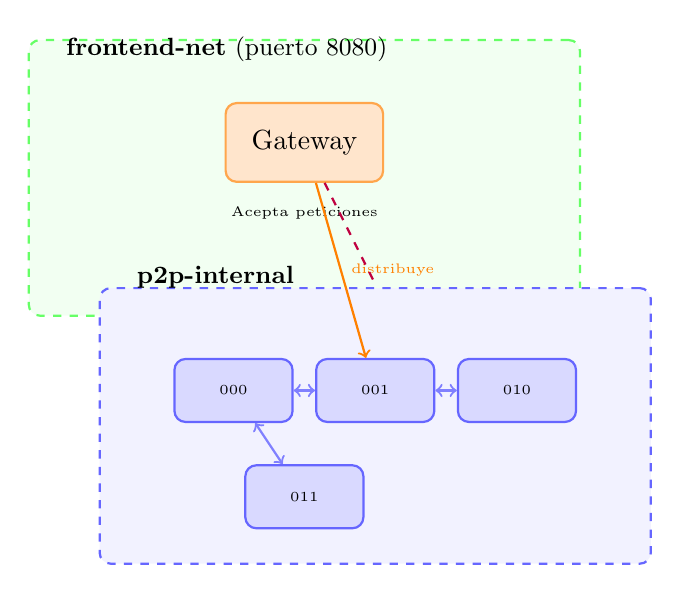
\begin{tikzpicture}[scale=0.9]
  \tikzstyle{net}=[rectangle, draw, thick, dashed, minimum width=7cm, minimum height=3.5cm, rounded corners]
  \tikzstyle{container}=[rectangle, draw=blue!60, fill=blue!15, thick, minimum width=1.5cm, minimum height=0.8cm, rounded corners]
  \tikzstyle{gateway}=[rectangle, draw=orange!70, fill=orange!20, thick, minimum width=2cm, minimum height=1cm, rounded corners]
  
  % Red frontend
  \node[net, draw=green!60, fill=green!5] (front) at (1,5) {};
  \node[above right, font=\small] at (-2.5,6.5) {\textbf{frontend-net} (puerto 8080)};
  \node[gateway] (gw) at (1,5.5) {Gateway};
  \node[font=\tiny] at (1,4.5) {Acepta peticiones};
  
  % Red P2P interna
  \node[net, draw=blue!60, fill=blue!5] (p2p) at (2,1.5) {};
  \node[above right, font=\small] at (-1.5,3.3) {\textbf{p2p-internal}};
  \node[container] (p1) at (0,2) {\tiny 000};
  \node[container] (p2) at (2,2) {\tiny 001};
  \node[container] (p3) at (4,2) {\tiny 010};
  \node[container] (p4) at (1,0.5) {\tiny 011};
  
  % Conexiones
  \draw[<->, thick, blue!50] (p1) -- (p2);
  \draw[<->, thick, blue!50] (p2) -- (p3);
  \draw[<->, thick, blue!50] (p1) -- (p4);
  \draw[->, thick, orange] (gw) -- node[right, font=\tiny] {distribuye} (p2);
  
  % Gateway en ambas redes
  \draw[thick, dashed, purple] (gw) -- (2,3.5);
\end{tikzpicture}
\caption{Distribución en dos redes Docker: gateway conecta frontend-net (pública) con p2p-internal (privada)}
\label{fig:docker-deploy}
\end{figure}

\subsection{Ventajas del diseño}

\begin{itemize}
  \item \textbf{Aislamiento}: Peers protegidos en red interna sin exposición directa
  \item \textbf{Escalabilidad}: Nuevos peers se agregan solo a \texttt{p2p-internal}
  \item \textbf{Punto de entrada único}: Gateway gestiona autenticación y balanceo
  \item \textbf{Separación de responsabilidades}: Frontend vs lógica P2P distribuida
\end{itemize}

\section{Procesos y patrones de diseño}

Cada nodo peer ejecuta uno o más procesos que proporcionan servicios especializados: un servicio de almacenamiento gestiona los datos locales y réplicas, un servicio de red se encarga del routing y escucha de conexiones entrantes, y un servicio de manejo de peticiones procesa las solicitudes tanto propias como de otros nodos. Si el sistema implementa lógica de balanceo o coordinación, esta puede residir como un módulo separado o subproceso dentro de algunos peers, ejecutándose de forma redundante para evitar puntos únicos de fallo.

En términos de concurrencia, cada nodo utiliza hilos o programación asíncrona (async I/O) para manejar múltiples conexiones y peticiones simultáneas sin bloqueos. El sistema adopta un patrón de diseño basado en concurrencia, asincronía y arquitectura dirigida por eventos (event-driven) con paso de mensajes (message-passing). Este enfoque es especialmente adecuado para sistemas distribuidos de red donde la latencia variable y las operaciones I/O dominan el tiempo de ejecución.

\subsection{Arquitectura interna de un nodo peer}

\begin{figure}[H]
\centering
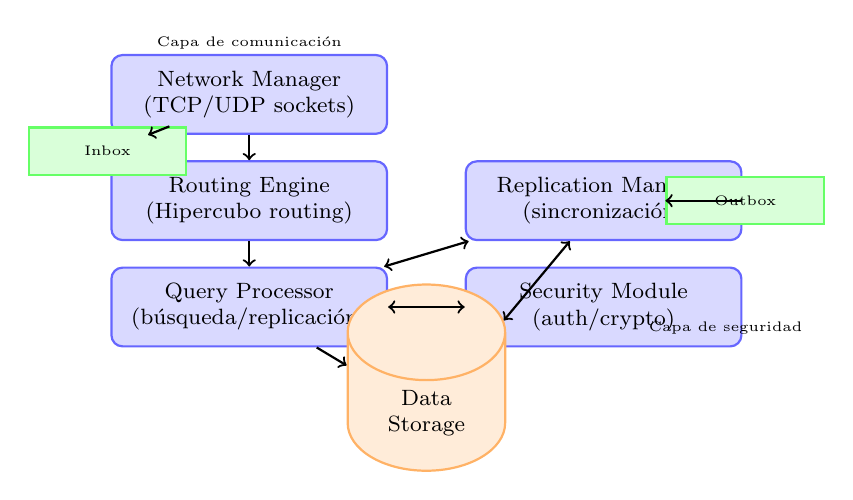
\begin{tikzpicture}[scale=0.9, node distance=1.5cm]
  \tikzstyle{component}=[rectangle, draw=blue!60, fill=blue!15, thick, minimum width=3.5cm, minimum height=1cm, rounded corners, font=\footnotesize, align=center]
  \tikzstyle{storage}=[cylinder, draw=orange!60, fill=orange!15, thick, minimum width=2cm, minimum height=1.2cm, shape border rotate=90, font=\footnotesize, align=center]
  \tikzstyle{queue}=[rectangle, draw=green!60, fill=green!15, thick, minimum width=2cm, minimum height=0.6cm, font=\tiny]
  
  % Componentes principales
  \node[component] (net) at (0,4) {Network Manager\\(TCP/UDP sockets)};
  \node[component] (route) at (0,2.5) {Routing Engine\\(Hipercubo routing)};
  \node[component] (query) at (0,1) {Query Processor\\(búsqueda/replicación)};
  \node[component] (rep) at (5,2.5) {Replication Manager\\(sincronización)};
  \node[component] (sec) at (5,1) {Security Module\\(auth/crypto)};
  
  % Almacenamiento
  \node[storage] (store) at (2.5,-0.5) {Data\\Storage};
  
  % Colas de mensajes
  \node[queue] (q1) at (-2,3.2) {Inbox};
  \node[queue] (q2) at (7,2.5) {Outbox};
  
  % Conexiones
  \draw[->, thick] (net) -- (route);
  \draw[->, thick] (route) -- (query);
  \draw[->, thick] (query) -- (store);
  \draw[<->, thick] (query) -- (rep);
  \draw[<->, thick] (query) -- (sec);
  \draw[->, thick] (q1) -- (net);
  \draw[->, thick] (rep) -- (q2);
  \draw[<->, thick] (store) -- (rep);
  
  % Etiquetas
  \node[above, font=\tiny] at (0,4.5) {Capa de comunicación};
  \node[right, font=\tiny] at (5.5,0.7) {Capa de seguridad};
\end{tikzpicture}
\caption{Arquitectura modular de un nodo peer: actúa como cliente (Query Processor inicia búsquedas) y servidor (Network Manager atiende peticiones)}
\label{fig:peer-architecture}
\end{figure}

\subsection{Patrones de diseño aplicados}

\begin{description}
  \item[Event-Driven Architecture] — Cada componente reacciona a eventos (llegada de mensajes, timeouts, cambios de estado)
  \item[Message Passing] — Comunicación entre componentes mediante colas de mensajes asíncronas
  \item[Reactor Pattern] — Event loop que multiplexea I/O de múltiples sockets
  \item[Strategy Pattern] — Algoritmos de routing y replicación intercambiables
  \item[Observer Pattern] — Notificación de cambios de estado de red a componentes interesados
\end{description}

\subsection{Modelo de concurrencia}

\begin{figure}[H]
\centering
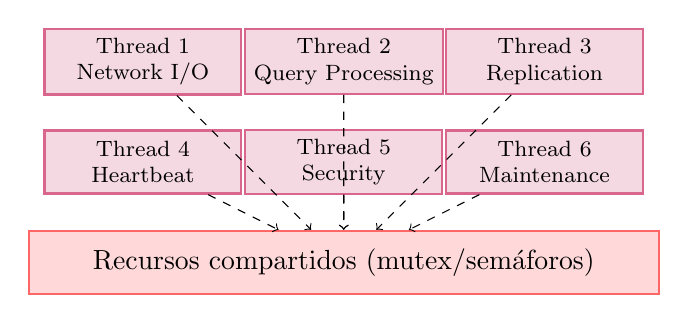
\begin{tikzpicture}[scale=0.85]
  \tikzstyle{thread}=[rectangle, draw=purple!60, fill=purple!15, thick, minimum width=2.5cm, minimum height=0.8cm, font=\footnotesize, align=center]
  
  \node[thread] (t1) at (0,3) {Thread 1\\Network I/O};
  \node[thread] (t2) at (3,3) {Thread 2\\Query Processing};
  \node[thread] (t3) at (6,3) {Thread 3\\Replication};
  \node[thread] (t4) at (0,1.5) {Thread 4\\Heartbeat};
  \node[thread] (t5) at (3,1.5) {Thread 5\\Security};
  \node[thread] (t6) at (6,1.5) {Thread 6\\Maintenance};
  
  % Recursos compartidos
  \node[rectangle, draw=red!60, fill=red!15, thick, minimum width=8cm, minimum height=0.8cm] (shared) at (3,0) {Recursos compartidos (mutex/semáforos)};
  
  \draw[->, dashed] (t1) -- (shared);
  \draw[->, dashed] (t2) -- (shared);
  \draw[->, dashed] (t3) -- (shared);
  \draw[->, dashed] (t4) -- (shared);
  \draw[->, dashed] (t5) -- (shared);
  \draw[->, dashed] (t6) -- (shared);
\end{tikzpicture}
\caption{Modelo de threads para manejo concurrente de operaciones}
\label{fig:concurrency}
\end{figure}

\section{Comunicación entre nodos}

\subsection{Modelo de comunicación por capas}

El sistema implementa una \textbf{arquitectura en capas} para la comunicación que separa las responsabilidades en tres niveles. La \textbf{capa de aplicación} define un protocolo de mensajería de alto nivel con mensajes como \texttt{REQUEST}, \texttt{RESPONSE}, \texttt{REPLICATE} y \texttt{HEARTBEAT}. Esta capa contiene la lógica de routing y búsqueda basada en la topología hipercubo, así como la gestión de sesiones y estado de transacciones. Cada peer interpreta estos mensajes y toma decisiones sobre cómo procesarlos o reenviarlos.

La \textbf{capa de transporte} utiliza sockets TCP para comunicación confiable en operaciones que requieren entrega garantizada, como transferencia de datos y replicación. Para mensajes de control de baja latencia que toleran pérdidas ocasionales, como heartbeats y descubrimiento de vecinos, se emplean sockets UDP. Esta capa también gestiona conexiones persistentes entre vecinos lógicos, manteniendo un pool de conexiones activas para minimizar la latencia de establecimiento.

La \textbf{capa de red} utiliza routing IP estándar sobre Internet. Es importante destacar que la topología overlay hipercubo es completamente independiente de la red física subyacente: dos nodos que son vecinos lógicos en el hipercubo pueden estar físicamente en diferentes continentes, mientras que nodos físicamente cercanos pueden no ser vecinos lógicos.

\subsection{Tipos de comunicación}

\subsubsection{Comunicación peer-to-peer directa}
Los nodos se comunican directamente mediante sockets TCP/UDP sin intermediarios. Cada peer mantiene conexiones activas con sus $d$ vecinos lógicos determinados por la topología hipercubo, lo que garantiza que cualquier peer pueda ser alcanzado en máximo $d$ saltos. Para operaciones síncronas como consultas de datos, se utiliza un modelo petición-respuesta (request-reply) donde el peer cliente espera una respuesta del peer servidor. Para operaciones asíncronas como replicación de datos y notificaciones de cambios de estado, se emplea mensajería asíncrona donde el emisor no bloquea esperando confirmación inmediata.

\subsubsection{Comunicación cliente-sistema}
Las aplicaciones externas que no forman parte de la red P2P (y por tanto no actúan como servidores) pueden acceder al sistema de dos formas. Pueden conectarse a través de un gateway que actúa como punto de entrada y balanceador de carga, redirigiendo peticiones a la red P2P interna. También un cliente externo puede comunicarse directamente con cualquier peer específico. En ambos casos, el cliente externo solo actúa como cliente, a diferencia de los peers que simultáneamente son clientes y servidores.

\subsection{Protocolo de mensajería}
Se definen los siguientes tipos de mensajes:

\begin{table}[H]
\centering
\begin{tabularx}{\textwidth}{|l|X|}
\hline
\textbf{Mensaje} & \textbf{Descripción} \\ \hline
\texttt{QUERY(key, ttl, origin)} & Búsqueda de dato con clave \texttt{key}, tiempo de vida \texttt{ttl}, nodo origen \\ \hline
\texttt{QUERY\_HIT(key, data, holder)} & Respuesta con el dato encontrado y nodo que lo posee \\ \hline
\texttt{STORE(key, data, replicas)} & Almacenar dato con número de réplicas especificado \\ \hline
\texttt{REPLICATE(key, data, target)} & Replicar dato hacia nodo objetivo \\ \hline
\texttt{PING / PONG} & Verificación de disponibilidad entre vecinos \\ \hline
\texttt{JOIN(node\_id, address)} & Notificación de unión de nuevo nodo \\ \hline
\texttt{LEAVE(node\_id)} & Notificación de salida de nodo \\ \hline
\end{tabularx}
\caption{Tipos de mensajes del protocolo P2P}
\label{tab:messages}
\end{table}

\subsection{Algoritmo de routing basado en distancia Hamming}
Para enviar un mensaje desde el nodo \(A\) al nodo \(B\):

\begin{algorithm}[H]
\caption{Routing en hipercubo}
\begin{algorithmic}[1]
\State \textbf{Input:} nodo actual $current$, nodo destino $target$
\State \textbf{Output:} siguiente salto en la ruta
\State $diff \gets current \oplus target$ \Comment{XOR bit a bit}
\If{$diff = 0$}
    \State \Return $target$ \Comment{Ya llegamos}
\EndIf
\State $bit \gets$ primer bit en 1 de $diff$ (de derecha a izquierda)
\State $next \gets current$ con el bit $bit$ invertido
\State \Return $next$
\end{algorithmic}
\end{algorithm}

\textbf{Ejemplo}: Para ilustrar el routing desde el nodo 000 al nodo 111, primero calculamos la diferencia: $diff = 000 \oplus 111 = 111$, lo que indica que difieren en los tres bits. El algoritmo invierte el bit menos significativo primero, moviendo de $000 \rightarrow 001$. Desde 001, la nueva diferencia es $diff = 001 \oplus 111 = 110$, por lo que invertimos el siguiente bit: $001 \rightarrow 011$. Finalmente, desde 011 calculamos $diff = 011 \oplus 111 = 100$ e invertimos el bit más significativo: $011 \rightarrow 111$, alcanzando el destino en exactamente 3 saltos (igual a la distancia Hamming entre ambos nodos).

\section{Coordinación y sincronización}

\subsection{Modelo de coordinación}

\subsubsection{Desacoplamiento temporal y referencial}

El sistema implementa diferentes niveles de acoplamiento según el tipo de operación:

\begin{table}[H]
\centering
\begin{tabularx}{\textwidth}{|l|X|X|}
\hline
\textbf{Operación} & \textbf{Acoplamiento temporal} & \textbf{Acoplamiento referencial} \\ \hline
Consulta directa & Acoplado (síncrono) & Acoplado (peer específico) \\ \hline
Replicación & Desacoplado (asíncrono) & Acoplado (réplicas específicas) \\ \hline
Búsqueda flooding & Desacoplado & Parcialmente desacoplado \\ \hline
Heartbeat & Desacoplado & Acoplado (vecinos) \\ \hline
\end{tabularx}
\caption{Niveles de acoplamiento por tipo de operación}
\label{tab:coupling}
\end{table}

El sistema implementa dos modos principales de comunicación con diferentes características de acoplamiento. La \textbf{comunicación directa} es temporalmente acoplada, lo que significa que ambos nodos (emisor y receptor) deben estar activos simultáneamente para completar la interacción. También es referencialmente acoplada porque el emisor conoce explícitamente la identidad del receptor. Este modo se utiliza para consultas síncronas donde se espera una respuesta inmediata y para transferencias de datos que requieren confirmación.

Por otro lado, la \textbf{comunicación basada en eventos} es temporalmente desacoplada, permitiendo que publicación y suscripción ocurran en momentos diferentes sin requerir sincronía estricta. También es referencialmente desacoplada ya que los publicadores no necesitan conocer la identidad de los suscriptores. Este patrón se emplea para notificaciones de cambios de estado, detección de fallos y propagación de eventos que múltiples nodos pueden consumir.

\subsection{Sincronización de acciones}

\subsubsection{Protocolo de sincronización para operaciones distribuidas}

\textbf{Protocolo de timestamps de Lamport:} El sistema utiliza relojes lógicos para establecer un ordenamiento parcial de eventos distribuidos. Cada nodo mantiene un contador $L_i$ que se incrementa en cada evento local. Cuando un nodo envía un mensaje, primero incrementa su reloj ($L_i := L_i + 1$) y adjunta este timestamp al mensaje. Al recibir un mensaje con timestamp $T$, el nodo receptor actualiza su reloj tomando el máximo entre su valor actual y el recibido, luego lo incrementa: $L_i := \max(L_i, T) + 1$. Este mecanismo garantiza que si un evento $a$ causalmente precede a un evento $b$, entonces el timestamp de $a$ será menor que el de $b$. Para resolver empates cuando dos eventos tienen el mismo timestamp, se utiliza el identificador del nodo como criterio de desempate: $(T_1, node_1) < (T_2, node_2)$ si $T_1 < T_2$, o si $T_1 = T_2$ y $node_1 < node_2$.

\subsection{Toma de decisiones distribuidas}

\subsubsection{Consenso para operaciones críticas}

\textbf{Escenario:} Decidir qué nodo se encarga de una tarea (ej: convertirse en coordinador de zona).

\textbf{Algoritmo de elección de líder (simplificado):}
\begin{enumerate}
  \item Cuando se detecta ausencia de coordinador, cada nodo calcula prioridad: \\
  $P_i = h(\text{node\_id}_i, \text{load}_i, \text{uptime}_i)$
  \item Cada nodo anuncia su prioridad a sus vecinos
  \item Nodo con mayor prioridad y confirmación de $\geq 2/3$ vecinos se designa líder
  \item Líder anuncia su rol a toda la red mediante flooding
\end{enumerate}

\textbf{Consenso para cambios de configuración:}
\begin{itemize}
  \item Cambios críticos (ej: modificar factor de replicación) requieren consenso
  \item Se usa votación de mayoría simple o algoritmo Raft simplificado
  \item Solo se aplica cambio si $> 50\%$ de nodos activos aprueban
\end{itemize}

\section{Localización y nombrado de datos / recursos}

Cada dato en el sistema tiene un identificador global único (ID o hash criptográfico) que lo distingue de otros elementos. El mecanismo de localización aprovecha la topología overlay del hipercubo combinada con lógica inteligente de búsqueda y routing. El sistema ofrece tres estrategias principales de localización.

La \textbf{búsqueda mediante reenvío} funciona cuando un peer recibe una petición de dato que no posee localmente: reenvía la consulta a sus vecinos lógicos, quienes a su vez propagan la búsqueda hasta encontrar una réplica del dato solicitado. La \textbf{búsqueda dirigida} utiliza heurísticas para optimizar el proceso, realizando encaminamiento preferente hacia nodos "más cercanos" según distancia de Hamming, seleccionando nodos con menor carga actual, o priorizando nodos con alto historial de disponibilidad.

\subsection{Estrategias de localización de datos}

\subsubsection{Estrategia 1: Búsqueda por inundación controlada (Flooding)}
\begin{algorithm}[H]
\caption{Búsqueda por flooding con TTL}
\begin{algorithmic}[1]
\State \textbf{Input:} $key$ (clave del dato), $ttl$ (tiempo de vida)
\State \textbf{Output:} dato encontrado o NULL
\If{dato con $key$ está en almacenamiento local}
    \State \Return dato
\EndIf
\If{$ttl \leq 0$}
    \State \Return NULL
\EndIf
\State Enviar \texttt{QUERY($key$, $ttl-1$)} a todos los vecinos
\State Esperar respuestas con timeout
\State \Return primera respuesta válida o NULL
\end{algorithmic}
\end{algorithm}

\subsubsection{Estrategia 2: Asignación determinística basada en hash}
Asignar cada dato al nodo cuya dirección es más cercana al hash del dato:
$$\text{nodo\_destino} = \arg\min_{i \in \text{nodos}} d_H(\text{hash}(key) \mod 2^d, i)$$
donde $d_H$ es la distancia de Hamming.

\textbf{Ejemplo} (hipercubo $d=3$): Consideremos un dato cuyo hash es 42. Para mapearlo al espacio de direcciones de dimensión 3, calculamos $42 \mod 8 = 2$, que en binario es 010. Por lo tanto, este dato se almacena preferentemente en el nodo con dirección 010, y sus réplicas se distribuyen en nodos vecinos para garantizar disponibilidad y tolerancia a fallos.

\begin{figure}[H]
\centering
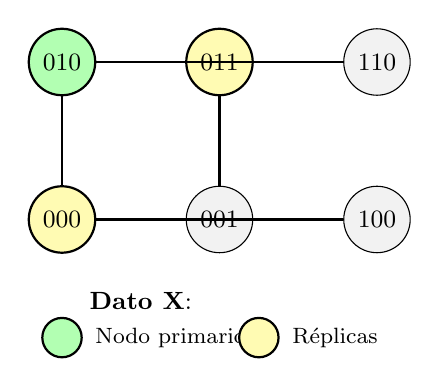
\begin{tikzpicture}[scale=1.0]
  \tikzstyle{node}=[circle, draw, minimum size=0.8cm, font=\small]
  \tikzstyle{primary}=[fill=green!30, thick]
  \tikzstyle{replica}=[fill=yellow!30, thick]
  \tikzstyle{normal}=[fill=gray!10]
  
  % Hipercubo simplificado 2D para visualización
  \node[node, primary] (n010) at (0,2) {010};
  \node[node, replica] (n000) at (0,0) {000};
  \node[node, replica] (n011) at (2,2) {011};
  \node[node, normal] (n001) at (2,0) {001};
  \node[node, normal] (n110) at (4,2) {110};
  \node[node, normal] (n100) at (4,0) {100};
  
  \draw[-, thick] (n010) -- (n000);
  \draw[-, thick] (n010) -- (n011);
  \draw[-, thick] (n000) -- (n001);
  \draw[-, thick] (n011) -- (n001);
  \draw[-, thick] (n010) -- (n110);
  \draw[-, thick] (n000) -- (n100);
  
  % Leyenda
  \node[below] at (1,-0.8) {\small \textbf{Dato X}:};
  \node[node, primary, minimum size=0.5cm] at (0,-1.5) {};
  \node[right, font=\footnotesize] at (0.3,-1.5) {Nodo primario};
  \node[node, replica, minimum size=0.5cm] at (2.5,-1.5) {};
  \node[right, font=\footnotesize] at (2.8,-1.5) {Réplicas};
\end{tikzpicture}
\caption{Distribución de dato X: nodo primario 010 con réplicas en vecinos 000 y 011}
\label{fig:data-location}
\end{figure}

\section{Distribución, replicación y consistencia de datos}

El sistema implementa replicación de datos donde cada elemento puede tener $k$ réplicas en diferentes nodos (típicamente $k = 2$ o $k = 3$) para garantizar tolerancia a fallos y alta disponibilidad. El protocolo de replicación funciona asignando, al momento de insertar un dato, las réplicas a nodos distintos que idealmente estén "lejanos" en la topología hipercubo. Esta distancia lógica maximiza la probabilidad de que las réplicas sobrevivan a fallos correlacionados.

Respecto a la consistencia, los datos son inmutables, entonces  el problema se simplifica ya que no hay sincronización de actualizaciones.

\subsection{Estrategia de replicación}
Para un factor de replicación $k=3$, al almacenar un dato en el nodo primario $N_p$, el sistema selecciona $k-1 = 2$ nodos adicionales para almacenar réplicas. Los criterios de selección incluyen maximizar la distancia de Hamming entre réplicas para lograr dispersión geográfica lógica, preferir nodos con baja carga actual para balancear el almacenamiento, y priorizar nodos con alta disponibilidad histórica según métricas de uptime. Una vez seleccionados los nodos, el sistema envía mensajes \texttt{REPLICATE} y espera confirmación de almacenamiento antes de considerar la operación completa.

\begin{figure}[H]
\centering
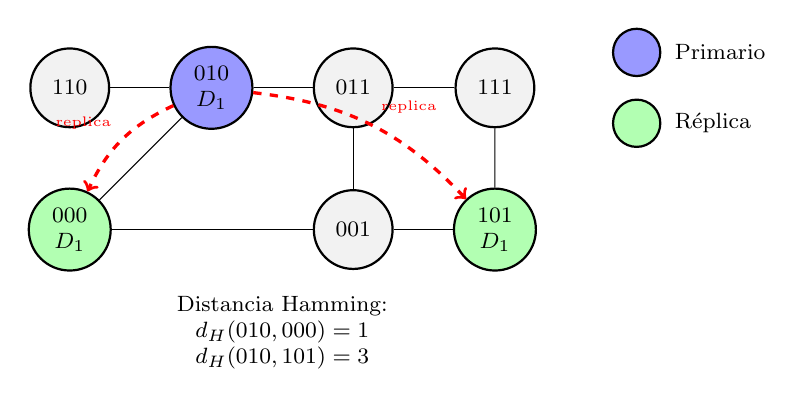
\begin{tikzpicture}[scale=0.9]
  \tikzstyle{node}=[circle, draw, thick, minimum size=1cm, font=\footnotesize, align=center]
  \tikzstyle{primary}=[fill=blue!40]
  \tikzstyle{replica}=[fill=green!30]
  \tikzstyle{normal}=[fill=gray!10]
  
  % Hipercubo 3D simplificado
  \node[node, primary] (p) at (0,2) {010\\$D_1$};
  \node[node, replica] (r1) at (-2,0) {000\\$D_1$};
  \node[node, normal] (n1) at (2,2) {011};
  \node[node, replica] (r2) at (4,0) {101\\$D_1$};
  \node[node, normal] (n2) at (2,0) {001};
  \node[node, normal] (n3) at (-2,2) {110};
  \node[node, normal] (n4) at (4,2) {111};
  
  % Conexiones
  \draw[-] (p) -- (n1);
  \draw[-] (p) -- (r1);
  \draw[-] (p) -- (n3);
  \draw[-] (r1) -- (n2);
  \draw[-] (n1) -- (n2);
  \draw[-] (n1) -- (n4);
  \draw[-] (r2) -- (n4);
  \draw[-] (r2) -- (n2);
  
  % Flechas de replicación
  \draw[->, very thick, red, dashed] (p) to[bend right=20] node[midway, above left] {\tiny replica} (r1);
  \draw[->, very thick, red, dashed] (p) to[bend left=20] node[midway, above right] {\tiny replica} (r2);
  
  % Leyenda
  \node[node, primary, minimum size=0.6cm] at (6,2.5) {};
  \node[right, font=\footnotesize] at (6.4,2.5) {Primario};
  \node[node, replica, minimum size=0.6cm] at (6,1.5) {};
  \node[right, font=\footnotesize] at (6.4,1.5) {Réplica};
  
  % Información de distancias
  \node[below, font=\footnotesize, align=center] at (1,-0.8) {
    Distancia Hamming:\\
    $d_H(010, 000) = 1$\\
    $d_H(010, 101) = 3$
  };
\end{tikzpicture}
\caption{Replicación de dato $D_1$ con factor $k=3$: nodo primario 010 y réplicas en 000 y 101}
\label{fig:replication}
\end{figure}

\subsection{Protocolo de consistencia eventual}

\begin{algorithm}[H]
\caption{Actualización con consistencia eventual}
\begin{algorithmic}[1]
\State \textbf{Input:} $key$, $new\_value$, $timestamp$
\State Actualizar valor local si $timestamp$ es más reciente
\State Obtener lista de réplicas para $key$
\For{cada réplica $r$ en lista}
    \State Enviar \texttt{UPDATE($key$, $new\_value$, $timestamp$)} a $r$
    \State No esperar confirmación (asíncrono)
\EndFor
\State Programar verificación de consistencia periódica
\end{algorithmic}
\end{algorithm}

\subsection{Modelo de consistencia}

El sistema adopta un modelo de consistencia eventual con las siguientes características. Para operaciones de \textbf{lectura}, el sistema acepta respuestas de cualquier réplica disponible, lo que significa que un cliente puede obtener una versión que no sea la más reciente si otras réplicas aún no han sido actualizadas

La \textbf{convergencia} entre réplicas está garantizada eventualmente mediante timestamps lógicos y mecanismos de anti-entropy que periódicamente detectan y corrigen divergencias.

\section{Tolerancia a fallos, robustez y dinámicas de red}

El sistema proporciona soporte integral para fallos parciales, incluyendo nodos que se desconectan temporalmente, nodos que fallan permanentemente, y la reincorporación de nodos nuevos o recuperados. La topología de hipercubo es fundamental para la resiliencia ya que ofrece múltiples rutas alternativas entre cualquier par de nodos, proporcionando redundancia natural ante fallos de nodos o enlaces individuales.

Cuando un nodo nuevo se une a la red o un nodo existente sale, es necesario reconfigurar las conexiones lógicas del sistema. Esto implica asignar o actualizar la dirección del nodo en el hipercubo, establecer o terminar conexiones con sus vecinos lógicos determinados por diferencias de un bit, reasignar réplicas si el nodo que falla era responsable de datos críticos, y actualizar las tablas de routing para reflejar la nueva topología.

El manejo de errores se implementa mediante múltiples estrategias complementarias. Se configuran timeouts para detectar nodos no responsivos, se reintentan peticiones fallidas dirigiéndolas hacia vecinos alternativos en la topología, y se implementa fallback automático a réplicas cuando el nodo primario no está disponible.

\subsection{Detección de fallos mediante Heartbeat}
\begin{algorithm}[H]
\caption{Protocolo Heartbeat para detección de fallos}
\begin{algorithmic}[1]
\State \textbf{Constantes:} $T_{heartbeat} = 5s$, $T_{timeout} = 15s$
\While{nodo está activo}
    \For{cada vecino $v$ en lista de vecinos}
        \State Enviar \texttt{PING} a $v$
        \If{no se recibe \texttt{PONG} en $T_{timeout}$}
            \State Marcar $v$ como fallido
            \State Notificar a otros vecinos sobre fallo de $v$
            \State Intentar reconexión o buscar reemplazo
        \EndIf
    \EndFor
    \State Esperar $T_{heartbeat}$
\EndWhile
\end{algorithmic}
\end{algorithm}

\subsection{Protocolo de incorporación de nuevo nodo (JOIN)}
\begin{figure}[H]
\centering
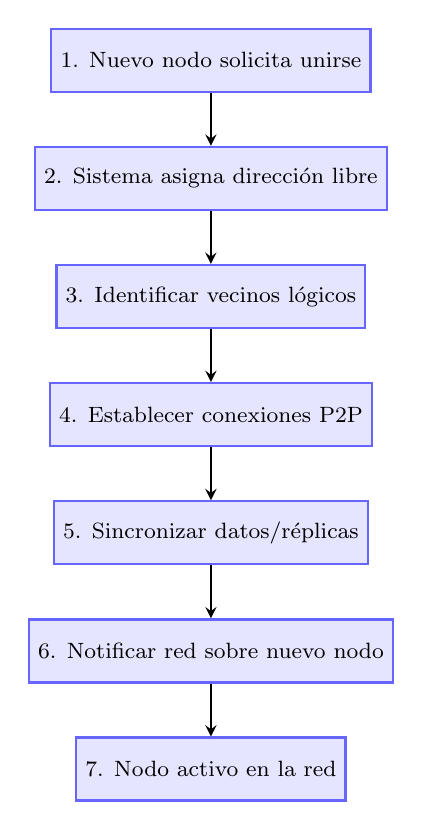
\begin{tikzpicture}[scale=0.8, node distance=1.5cm]
  \tikzstyle{process}=[rectangle, draw=blue!60, fill=blue!10, thick, minimum width=3cm, minimum height=0.8cm, font=\footnotesize, align=center]
  \tikzstyle{arrow}=[->, thick, >=stealth]
  
  \node[process] (s1) {1. Nuevo nodo solicita unirse};
  \node[process, below of=s1] (s2) {2. Sistema asigna dirección libre};
  \node[process, below of=s2] (s3) {3. Identificar vecinos lógicos};
  \node[process, below of=s3] (s4) {4. Establecer conexiones P2P};
  \node[process, below of=s4] (s5) {5. Sincronizar datos/réplicas};
  \node[process, below of=s5] (s6) {6. Notificar red sobre nuevo nodo};
  \node[process, below of=s6] (s7) {7. Nodo activo en la red};
  
  \draw[arrow] (s1) -- (s2);
  \draw[arrow] (s2) -- (s3);
  \draw[arrow] (s3) -- (s4);
  \draw[arrow] (s4) -- (s5);
  \draw[arrow] (s5) -- (s6);
  \draw[arrow] (s6) -- (s7);
\end{tikzpicture}
\caption{Proceso de incorporación de nuevo nodo a la red P2P}
\label{fig:join-protocol}
\end{figure}

\subsection{Manejo de fallo de nodo}
Cuando un nodo $N$ falla:

\begin{enumerate}
  \item \textbf{Detección}: Vecinos detectan fallo por timeout de heartbeat
  \item \textbf{Notificación}: Vecinos notifican al resto de la red
  \item \textbf{Reconexión}: Vecinos de $N$ se conectan entre sí para mantener conectividad
  \item \textbf{Re-replicación}: Datos con réplicas en $N$ se replican en otros nodos
  \item \textbf{Actualización de rutas}: Tablas de routing se actualizan
\end{enumerate}

\begin{figure}[H]
\centering
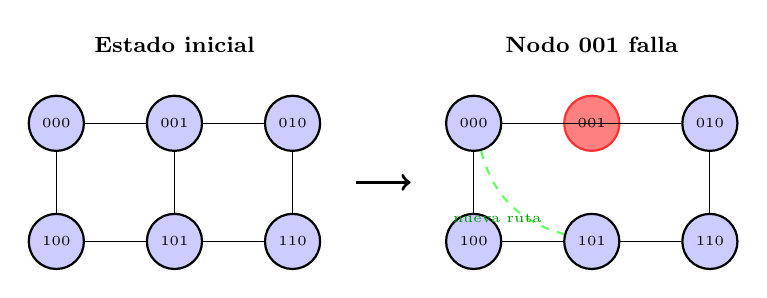
\begin{tikzpicture}[scale=1.0]
  % Estado inicial
  \begin{scope}
    \node[font=\footnotesize\bfseries] at (1.5,2.5) {Estado inicial};
    \tikzstyle{node}=[circle, draw, thick, minimum size=0.7cm, font=\tiny, fill=blue!20]
    \tikzstyle{failed}=[fill=red!50]
    
    \node[node] (a1) at (0,1.5) {000};
    \node[node] (b1) at (1.5,1.5) {001};
    \node[node] (c1) at (3,1.5) {010};
    \node[node] (d1) at (0,0) {100};
    \node[node] (e1) at (1.5,0) {101};
    \node[node] (f1) at (3,0) {110};
    
    \draw[-] (a1) -- (b1);
    \draw[-] (b1) -- (c1);
    \draw[-] (a1) -- (d1);
    \draw[-] (b1) -- (e1);
    \draw[-] (c1) -- (f1);
    \draw[-] (d1) -- (e1);
    \draw[-] (e1) -- (f1);
  \end{scope}
  
  % Flecha de transición
  \draw[->, very thick] (3.8,0.75) -- (4.5,0.75);
  
  % Estado después del fallo
  \begin{scope}[xshift=5.3cm]
    \node[font=\footnotesize\bfseries] at (1.5,2.5) {Nodo 001 falla};
    \tikzstyle{node}=[circle, draw, thick, minimum size=0.7cm, font=\tiny, fill=blue!20]
    \tikzstyle{failed}=[fill=red!50, draw=red!80]
    
    \node[node] (a2) at (0,1.5) {000};
    \node[node, failed] (b2) at (1.5,1.5) {001};
    \node[node] (c2) at (3,1.5) {010};
    \node[node] (d2) at (0,0) {100};
    \node[node] (e2) at (1.5,0) {101};
    \node[node] (f2) at (3,0) {110};
    
    \draw[-] (a2) -- (c2);
    \draw[-] (a2) -- (d2);
    \draw[-] (c2) -- (f2);
    \draw[-] (d2) -- (e2);
    \draw[-] (e2) -- (f2);
    \draw[-, dashed, thick, green!60] (a2) to[bend right=30] (e2);
    
    \node[font=\tiny, green!60!black] at (0.3,0.3) {nueva ruta};
  \end{scope}
\end{tikzpicture}
\caption{Reconfiguración de red tras fallo de nodo 001: rutas alternativas y reconexiones}
\label{fig:fault-tolerance}
\end{figure}

\subsection{Métricas de resiliencia}

Para un hipercubo de dimensión $d$, el sistema presenta características de resiliencia cuantificables. La \textbf{conectividad de nodo} es igual a $d$, lo que significa que cada nodo puede tolerar hasta $d$ fallos de vecinos antes de quedar desconectado de la red. Existen $d!$ (factorial de $d$) rutas alternativas posibles entre cualquier par de nodos, proporcionando múltiples caminos de routing ante fallos. El \textbf{tiempo de detección de fallo} está determinado por el timeout de heartbeat, configurado en $T_{timeout} = 15s$. El \textbf{tiempo de recuperación} tras un fallo es del orden de $O(d \cdot T_{message})$, donde $T_{message}$ es el tiempo promedio de entrega de mensaje, ya que la información de reconfiguración debe propagarse a través de $d$ saltos máximo.

\section{Seguridad, autenticación y autorización}

El sistema implementa múltiples capas de seguridad para proteger tanto los datos como la integridad de la red. Cada nodo posee una identidad única basada en criptografía de clave pública (par de claves pública/privada), lo que permite autenticación mutua entre peers antes de establecer comunicación. Toda la comunicación entre nodos se realiza mediante canales cifrados usando TLS (Transport Layer Security), protegiendo los datos en tránsito contra escuchas y manipulación.

El sistema implementa control de acceso mediante permisos que definen qué nodos pueden leer o escribir ciertos datos. Esto se logra usando firmas digitales para verificar autoriz ación, listas de control de acceso (ACLs) basadas en identidad de nodo, y certificados digitales que vinculan identidades con permisos específicos. Para mitigar la presencia de nodos maliciosos, el sistema emplea múltiples mecanismos: verificación de integridad mediante hashes criptográficos (SHA-256) y firmas digitales, sistemas de reputación que rastrean el comportamiento histórico de los nodos, validación de datos mediante consenso entre múltiples peers, limitación de privilegios siguiendo el principio de mínimo privilegio, y protección contra ataques Sybil mediante pruebas de identidad y restricción de nuevas incorporaciones.

\subsection{Modelo de seguridad por capas}

\begin{figure}[H]
\centering
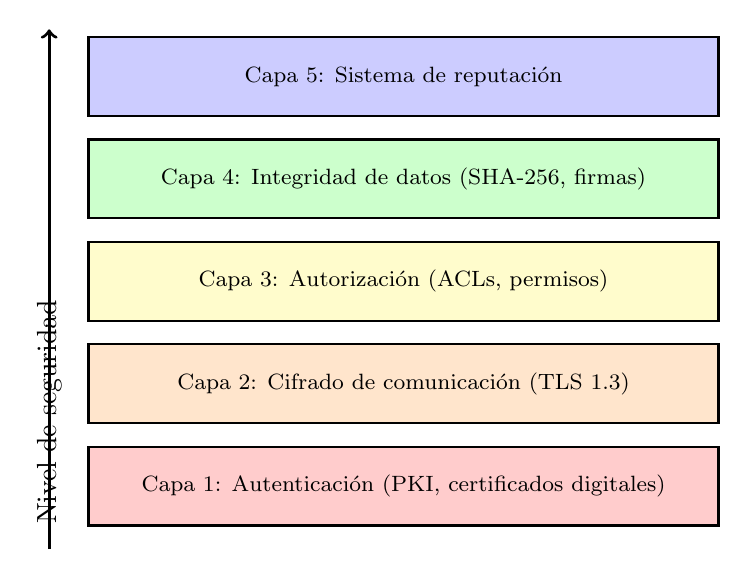
\begin{tikzpicture}[scale=1.0]
  \tikzstyle{layer}=[rectangle, draw, thick, minimum width=8cm, minimum height=1cm, font=\footnotesize]
  
  \node[layer, fill=red!20] (l1) at (0,0) {Capa 1: Autenticación (PKI, certificados digitales)};
  \node[layer, fill=orange!20] (l2) at (0,1.3) {Capa 2: Cifrado de comunicación (TLS 1.3)};
  \node[layer, fill=yellow!20] (l3) at (0,2.6) {Capa 3: Autorización (ACLs, permisos)};
  \node[layer, fill=green!20] (l4) at (0,3.9) {Capa 4: Integridad de datos (SHA-256, firmas)};
  \node[layer, fill=blue!20] (l5) at (0,5.2) {Capa 5: Sistema de reputación};
  
  \draw[->, very thick] (-4.5,-0.8) -- (-4.5,5.8) node[midway, left, rotate=90] {Nivel de seguridad};
\end{tikzpicture}
\caption{Arquitectura de seguridad por capas}
\label{fig:security-layers}
\end{figure}

\subsection{Protocolo de autenticación}

\begin{algorithm}[H]
\caption{Autenticación mutua entre peers}
\begin{algorithmic}[1]
\State \textbf{Nodo A quiere conectarse con Nodo B}
\State A genera nonce $N_A$ aleatorio
\State A $\rightarrow$ B: \texttt{HELLO}($ID_A$, $N_A$, $Cert_A$)
\State B verifica $Cert_A$ con autoridad certificadora
\If{$Cert_A$ es válido}
    \State B genera nonce $N_B$
    \State B $\rightarrow$ A: \texttt{CHALLENGE}($N_B$, $Sign_B(N_A)$, $Cert_B$)
    \State A verifica $Cert_B$ y $Sign_B(N_A)$
    \If{verificación exitosa}
        \State A $\rightarrow$ B: \texttt{RESPONSE}($Sign_A(N_B)$)
        \State B verifica $Sign_A(N_B)$
        \State \textbf{Conexión autenticada establecida}
        \State Establecer canal TLS con claves de sesión
    \EndIf
\EndIf
\end{algorithmic}
\end{algorithm}

\subsection{Control de acceso basado en permisos}

Cada dato tiene asociado un descriptor de seguridad:

\begin{table}[H]
\centering
\begin{tabularx}{0.9\textwidth}{|l|X|}
\hline
\textbf{Campo} & \textbf{Descripción} \\ \hline
\texttt{owner} & ID del nodo propietario del dato \\ \hline
\texttt{readers} & Lista de nodos con permiso de lectura \\ \hline
\texttt{writers} & Lista de nodos con permiso de escritura \\ \hline
\texttt{signature} & Firma digital del propietario \\ \hline
\texttt{hash} & Hash SHA-256 para verificar integridad \\ \hline
\texttt{timestamp} & Marca temporal de creación/modificación \\ \hline
\end{tabularx}
\caption{Descriptor de seguridad de datos}
\label{tab:security-descriptor}
\end{table}

\subsection{Sistema de reputación contra nodos maliciosos}

Cada nodo mantiene una tabla de reputación de sus vecinos que se actualiza continuamente según un modelo de promedio ponderado exponencial: $R_i(t+1) = \alpha \cdot R_i(t) + (1-\alpha) \cdot B_i(t)$, donde $R_i(t)$ representa la reputación del nodo $i$ en el tiempo $t$, $B_i(t)$ captura el comportamiento reciente tomando valor $1$ para comportamiento bueno y $0$ para comportamiento malo, y $\alpha = 0.9$ es el factor de decaimiento que da mayor peso al historial. 

El sistema toma acciones diferenciadas según el nivel de reputación: nodos con $R_i > 0.8$ son considerados confiables y reciben prioridad alta en routing y almacenamiento; nodos con $0.5 < R_i \leq 0.8$ son tratados como normales sin privilegios especiales ni restricciones; nodos con $0.3 < R_i \leq 0.5$ son clasificados como sospechosos y sometidos a monitoreo aumentado; finalmente, nodos con $R_i \leq 0.3$ son bloqueados y desconectados de la red para proteger la integridad del sistema.

\subsection{Mitigación de ataques comunes}

\begin{table}[H]
\centering
\begin{tabularx}{\textwidth}{|l|X|X|}
\hline
\textbf{Ataque} & \textbf{Descripción} & \textbf{Mitigación} \\ \hline
Sybil & Crear múltiples identidades falsas & PKI + verificación de identidad + límite de nodos por IP \\ \hline
Eclipse & Aislar nodo víctima & Diversificación de conexiones + monitoreo de conectividad \\ \hline
Man-in-the-Middle & Interceptar comunicaciones & TLS 1.3 + autenticación mutua \\ \hline
Data poisoning & Insertar datos corruptos & Firmas digitales + verificación de hash + reputación \\ \hline
DDoS & Saturar nodos con peticiones & Rate limiting + listas negras + sistema de reputación \\ \hline
\end{tabularx}
\caption{Ataques comunes y mecanismos de mitigación}
\label{tab:attacks}
\end{table}

\section{Análisis de Calidad del Sistema}

\subsection{Propiedades del diseño}

El sistema presenta 4 propiedades fundamentales que caracterizan su arquitectura. La \textbf{descentralización} garantiza que no existe un punto central de fallo, ya que todos los nodos poseen capacidades equivalentes y pueden asumir cualquier rol necesario. La \textbf{redundancia} se manifiesta en múltiples rutas alternativas entre nodos y en la replicación de datos a través de múltiples nodos. La \textbf{escalabilidad} se logra mediante un crecimiento logarítmico tanto de los recursos requeridos por nodo como del diámetro de la red respecto al número total de nodos. La \textbf{flexibilidad} permite la incorporación y salida dinámica de nodos sin interrumpir el servicio. 

\subsection{Escalabilidad del diseño}

\begin{table}[H]
\centering
\begin{tabularx}{\textwidth}{|c|c|c|c|X|}
\hline
\textbf{Dimensión $d$} & \textbf{Nodos ($2^d$)} & \textbf{Diámetro} & \textbf{Vecinos/nodo} & \textbf{Escenario de uso} \\ \hline
3 & 8 & 3 & 3 & Prototipo/Testing \\ \hline
4 & 16 & 4 & 4 & Desarrollo \\ \hline
5 & 32 & 5 & 5 & Despliegue piloto \\ \hline
6 & 64 & 6 & 6 & Producción pequeña \\ \hline
7 & 128 & 7 & 7 & Producción media \\ \hline
8 & 256 & 8 & 8 & Producción grande \\ \hline
10 & 1024 & 10 & 10 & Escala empresarial \\ \hline
\end{tabularx}
\caption{Escalabilidad del hipercubo según dimensión}
\label{tab:scalability}
\end{table}

\textbf{Análisis}: La estructura hipercubo presenta características de escalabilidad excepcionales. El diámetro de la red crece logarítmicamente con el número de nodos según la fórmula $d = \log_2(N)$, lo que significa que duplicar el número de nodos solo incrementa el diámetro en uno. Cada nodo mantiene exactamente $\log_2(N)$ conexiones activas independientemente del tamaño total de la red, evitando que el overhead de conectividad crezca linealmente. Esto proporciona excelente escalabilidad para sistemas de hasta varios miles de nodos, ya que el overhead de comunicación permanece manejable para la mayoría de aplicaciones prácticas. Incluso con 1024 nodos (dimensión 10), cada nodo solo necesita mantener 10 conexiones y la distancia máxima entre nodos es de 10 saltos.

\subsection{Métricas de rendimiento esperadas}

\begin{table}[H]
\centering
\begin{tabularx}{\textwidth}{|l|X|c|}
\hline
\textbf{Métrica} & \textbf{Descripción} & \textbf{Objetivo} \\ \hline
Disponibilidad & Porcentaje de tiempo que el sistema está operativo & $> 99.5\%$ \\ \hline
Latencia de búsqueda & Tiempo promedio para localizar un dato & $< 500$ms \\ \hline
Tasa de éxito & Porcentaje de búsquedas exitosas & $> 95\%$ \\ \hline
Throughput & Consultas por segundo soportadas & $> 1000$ qps \\ \hline
Overhead de red & Mensajes adicionales vs óptimo teórico & $< 3x$ \\ \hline
MTTR & Tiempo promedio de recuperación tras fallo & $< 30$s \\ \hline
\end{tabularx}
\caption{Métricas de rendimiento del sistema}
\label{tab:performance-metrics}
\end{table}





\section{Conclusión}

Este documento ha presentado la especificación arquitectónica completa de un sistema distribuido P2P basado en topología hipercubo. El diseño prioriza cinco aspectos fundamentales para garantizar un sistema robusto y escalable. La \textbf{descentralización completa} elimina puntos únicos de fallo al distribuir uniformemente las responsabilidades entre todos los nodos peers, donde cada nodo actúa simultáneamente como cliente cuando solicita datos y como servidor cuando atiende peticiones de otros nodos. La \textbf{alta disponibilidad} se logra mediante replicación estratégica de datos en nodos lógicamente distantes y múltiples rutas alternativas que garantizan conectividad incluso ante fallos parciales. La \textbf{tolerancia a fallos} se implementa con detección automática de nodos caídos mediante heartbeats y mecanismos de recuperación que permiten reconexiones dinámicas. La \textbf{seguridad} abarca protocolos robustos de autenticación basados en PKI, cifrado de comunicaciones mediante TLS, y control de acceso granular con sistemas de reputación para mitigar nodos maliciosos. Finalmente, la \textbf{escalabilidad} se asegura mediante un crecimiento logarítmico de recursos por nodo, donde cada peer mantiene solo $\log_2(N)$ conexiones independientemente del tamaño total del sistema.

\section*{Referencias}
% Lista de referencias bibliográficas utilizadas
% Puedes formatearlas según el estilo que prefieras (IEEE, APA, etc.)
\begin{itemize}
  \item “Peer-to-Peer (P2P) Architecture – GeeksforGeeks” — definición y características del modelo P2P.  
  \item “Structured and Unstructured Peer-to-Peer Systems – GeeksforGeeks” — diferencias entre redes estructuradas y no estructuradas.  
  \item Artículos sobre overlays basados en hipercubo para sistemas P2P / distribuidos.  
\end{itemize}

\end{document}
